\documentclass{beamer}
 
\usepackage[utf8]{inputenc}
\usepackage{xcolor}
\definecolor{darkred}{rgb}{0.8,0,0} %Color of beaver theme
\usepackage[ruled,noend]{algorithm2e}
\usepackage{graphicx}
%\usepackage{sidecap}

\usetheme{Copenhagen}
\usecolortheme{beaver}

%%LINES
\newlength{\seplinewidth}
\newlength{\seplinesep}
\setlength{\seplinewidth}{0.02mm}
\setlength{\seplinesep}{1.4mm}
\colorlet{sepline}{darkred}
\newcommand*{\sepline}{%
  \par
  \vspace{\dimexpr\seplinesep+.5\parskip}%
  \cleaders\vbox{%
    \begingroup % because of color
      \color{sepline}%
      \hrule width\linewidth height\seplinewidth
    \endgroup
  }\vskip\seplinewidth
  \vspace{\dimexpr\seplinesep-.5\parskip}%
}
%%LINES
 
%Information to be included in the title page:
\title[One Table to Count Them All: Parallel Frequency Estimation on Single-Board Computers] %optional
{One Table to Count Them All: \\Parallel Frequency Estimation on Single-Board Computers}
 
%\subtitle{``A cache focused approach"}
 
\author[Kamer Kaya] % (optional, for multiple authors)
{\textcolor{darkred}{Kamer Kaya}}
 
\institute[Sabancı University] % (optional)
{
  \inst{}%
  Sabancı University, Turkey
  %Computer Science \& Engineering
}
 
\date[] % (optional)
{
%Euro-Par 2019 \\ %\noindent\makebox[\linewidth]{\rule{10cm}{0.4pt}}
%\vspace{-0.5cm}
\sepline
 {
 Joint work with: \\ 
 \vspace{4mm}
 \textcolor{darkred}{Fatih Taşyaran} \hspace{9mm} 
 \textcolor{darkred}{Kerem Yıldırır} \hspace{9mm} 
 \textcolor{darkred}{M. Kemal Taş} \\
 %\vspace{2mm}
 \hspace{-0ex}
 {\tiny Sabancı University} \hspace{9ex}
 {\tiny Sabancı University}  \hspace{9ex}
  {\tiny Sabancı University} 
 }
\sepline
 }
 

 
\begin{document}
 
\frame{\titlepage}
 
\begin{frame}
	\frametitle{Motivation and Context}
	\begin{itemize}
	\item Sketches are probabilistic data structures that can provide:
	\begin{itemize}
	\item approximate results within mathematically proven error bounds 
	\item while using orders of magnitude less memory than traditional approaches.
	\end{itemize}
	\item They are tailored for streaming data analysis on architectures even with limited memory such as single-board computers.
	\item Although these devices offer multiple cores, their caches are relatively small and a careful parallelization is required.

\end{itemize}
\end{frame}

\begin{frame}
	\frametitle{Motivation and Context}
		\begin{itemize}
	\item We propose an efficient hashing approach to compute multiple tabular hash functions at once,
	\item We carefully parallelize Count-Min Sketch on cache-limited, single board, multicore devices,
	\item We extend our approach for devices with heterogeneous cores.

\end{itemize}
\end{frame}

\begin{frame}
\frametitle{Count-Min Sketch}
\begin{itemize}
\item
{\it Count-Min Sketch}~(CMS) is a probabilistic sketch that helps to estimate the frequencies, i.e., the number of occurrences, of the items in a stream~\cite{cormode2005}. The frequency  information is crucial to find heavy-hitters or rare items and detecting anomalies~\cite{cormode2003,cormode2005}.
       
\item Given two parameters $\epsilon$ and $\delta$, a Count-Min Sketch is constructed as a two-dimensional counter table with 
$$d=\lceil \ln(1/\delta) \rceil$$ rows and $$w=\lceil e/\epsilon \rceil$$ columns.
     \end{itemize}
\end{frame}


\begin{frame}
\frametitle{Count-Min Sketch}  
    \begin{figure}[h]
                 \centering
            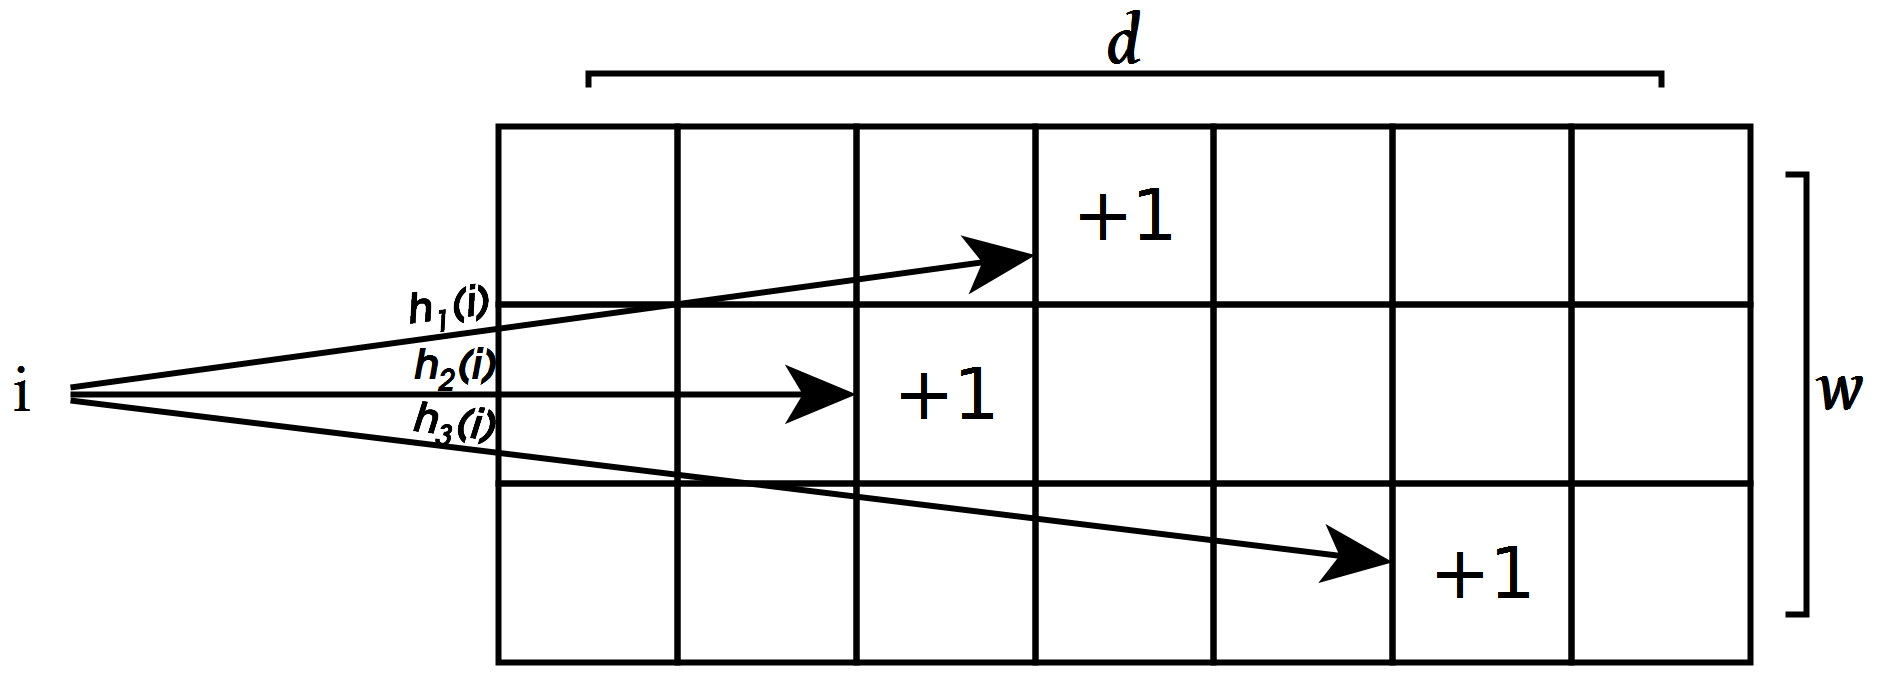
\includegraphics[scale=0.1]{cm_insert_illustration.png}
            \caption{Count-Min Sketch insert}
            \label{fig:b}
        \end{figure}
 \begin{itemize}
    \item Let $f_x$ be the frequency of an element in stream $S$ and $f'_x$ be the frequency returned by sketch query. \\
    \item With $d \times w$ memory, the sketch satisfies that $f_x \leq f'_x$ and $\Pr\left(f'_x \geq f_x + \epsilon N\right) \leq \delta.$
 \end{itemize}
\end{frame}

\begin{frame}
\frametitle{Algorithm I: Sequential CMS-Construction}
\begin{algorithm}[H]
	%\caption{\textsc{CMS-Construction}} 
	\KwIn{  $\epsilon$: error factor, $\delta$: error probability \\
		\hspace*{8ex}${\tt s}[.]$: a stream with $N$ elements from $n$ distinct elements \\ 
		\hspace*{8ex}$h_i(.)$: pairwise independent hash functions where for \\ 
		\hspace*{13ex}$1\leq i \leq d$,  $h_i$: $\mathcal{U} \rightarrow \{1,\cdots,w\}$ and $w = \lceil e/\epsilon \rceil$\\}
	\KwOut{ ${\tt cms}[.][.]$: a $d \times w$ counter sketch where $d = \lceil 1/\delta \rceil$ \\
	}
	
	${\tt cms}$[i][j] $ \leftarrow 0$ for $1 \leq i \leq d$ and $1 \leq j \leq w$
	
	\For{$i\leftarrow 1$ \KwTo $N$}{
		$x  \leftarrow s[i]$
		\For{$j\leftarrow 1$ \KwTo $d$}{
			$col \leftarrow h_j(x)$\\
			${\tt cms}$[j][$col$] $ \leftarrow {\tt cms}$[j][$col$] $ +1$
		}
	}
	\label{alg:cms_construct}
\end{algorithm}
\end{frame}




\begin{frame}
\frametitle{Tabulation Hash}
\begin{itemize}
\item CMS requires pairwise independent hash functions to provide the desired properties.
\item A separate hash function is used for each row of the CMS with a range equal  to the range of columns. 
\item We used tabulation hashing~\cite{zobrist1970} which has been recently analyzed by Patrascu and Thorup et al.~\cite{patrascu2012,thorup2017} which is as fast as classical multiply-mod-prime scheme, i.e. $(ax+b)$ mod $p$.
\end{itemize}
\end{frame}

\begin{frame}
\frametitle{Tabulation Hash}
		The spatial locality of the accessed tabulation elements can deteriorate the performance since each access is performed to a different table row~(of length 256). 
		Furthermore, there is no relation whatsoever among them to help us to fix the access pattern for all possible stream elements.

 \begin{figure}[H]
	\begin{minipage}[c]{0.40\textwidth}
	\hspace*{3ex} 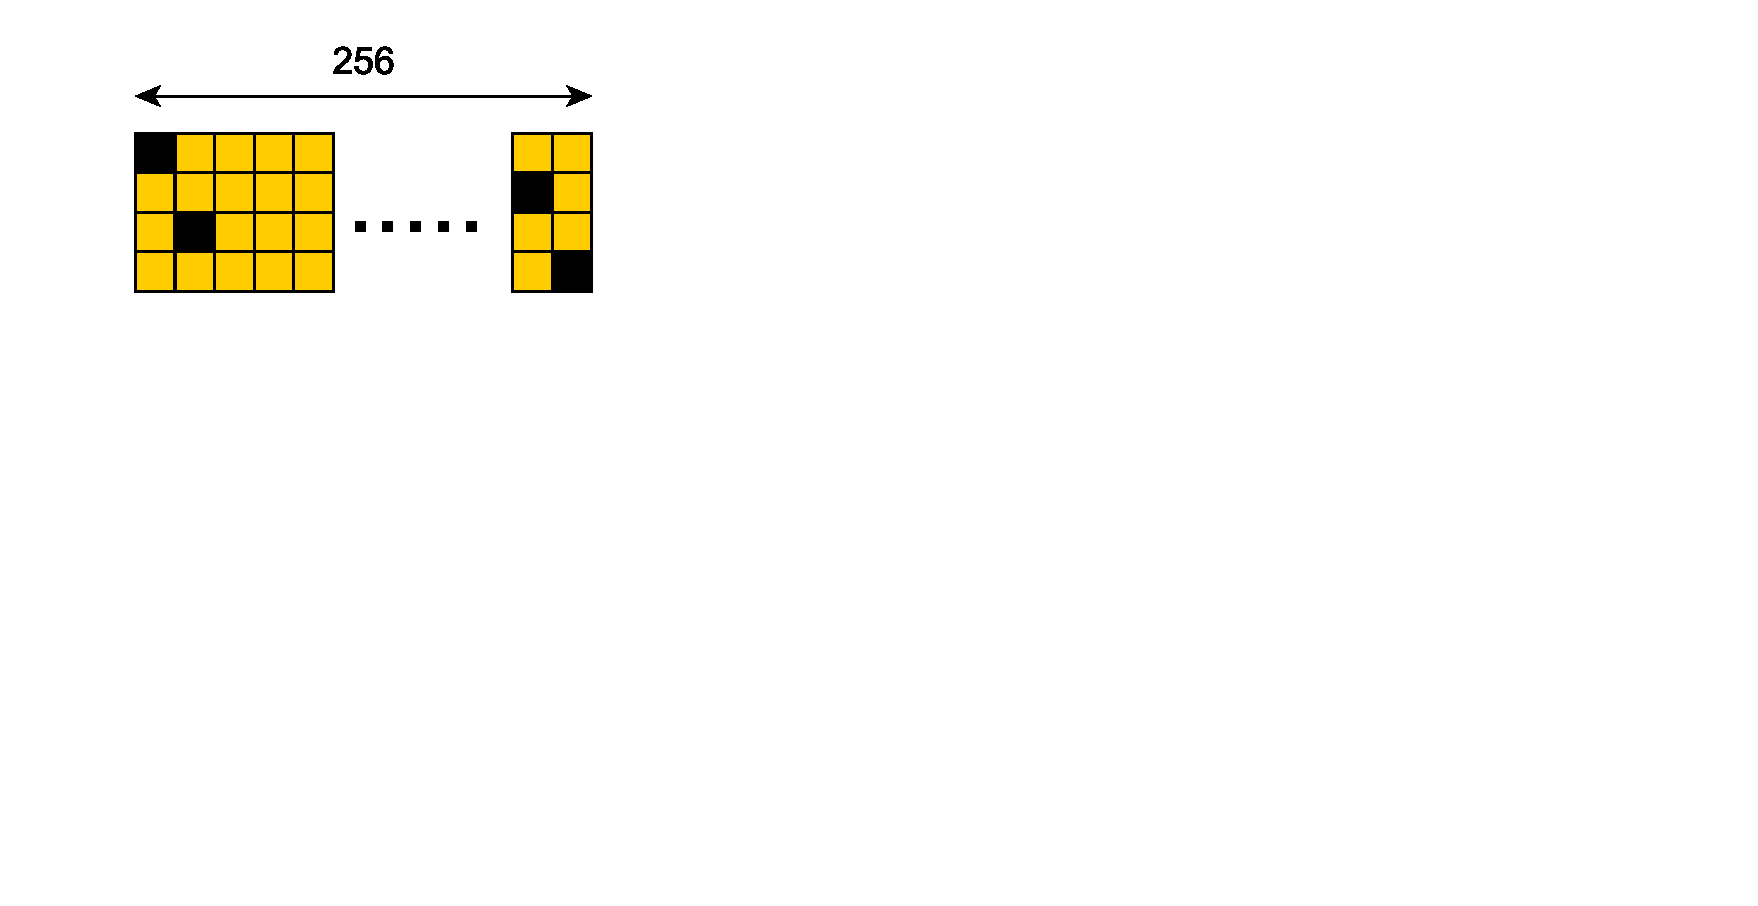
\includegraphics[scale=0.45]{single_tabular_access.pdf}
	\end{minipage}\hfill\hfill\hfill
	\begin{minipage}[c]{0.5\textwidth}
		\renewcommand{\baselinestretch}{0.9}
		\begin{algorithm}[H]
			\tiny
			\TitleOfAlgo{Naive Tabulation Hash\\}
			%\caption{\textsc{Naive Tabulation}}  
			\SetAlgoNoLine
			\KwIn{  \ \ $data$: 32-bit data to be hashed }
			\KwOut{ ${\tt h}$: hash value }
			$mask \leftarrow 0x000000ff$ \\
			$x \leftarrow data$ \\
			$h \leftarrow 0$ \\
			\For{$i\leftarrow 1$ \KwTo $4$}{
				$c \leftarrow x \& mask$ \\
				${\tt h}  \leftarrow  {h \oplus \tt table}[i][c]$\\
				$x \leftarrow x \gg 8$ \\
			}
		
			%}
			\label{algo:tabhash} 	
		\end{algorithm}
		\renewcommand{\baselinestretch}{1}
	\end{minipage}
\end{figure}
\end{frame}


\begin{frame}
	\frametitle{Merged Tabulation Hash}
	\begin{itemize}
	\item For many sketches, the same item is hashed more than once. 
	\item When tabulation hashing is used, this yields an interesting optimization; there exist multiple hash functions and hence, more than one hash table. 
	\item Although, the entries in a single table is accessed in a somehow irregular fashion, the accessed coordinates in all the tables are the same for different tables.
	\item Hence, the columns of the tables can be combined in an alternating fashion to utilize cache in a better way. 
		\end{itemize}
\end{frame}

\begin{frame}
	\frametitle{Merged Tabulation Hash}
		\begin{figure}[H]
			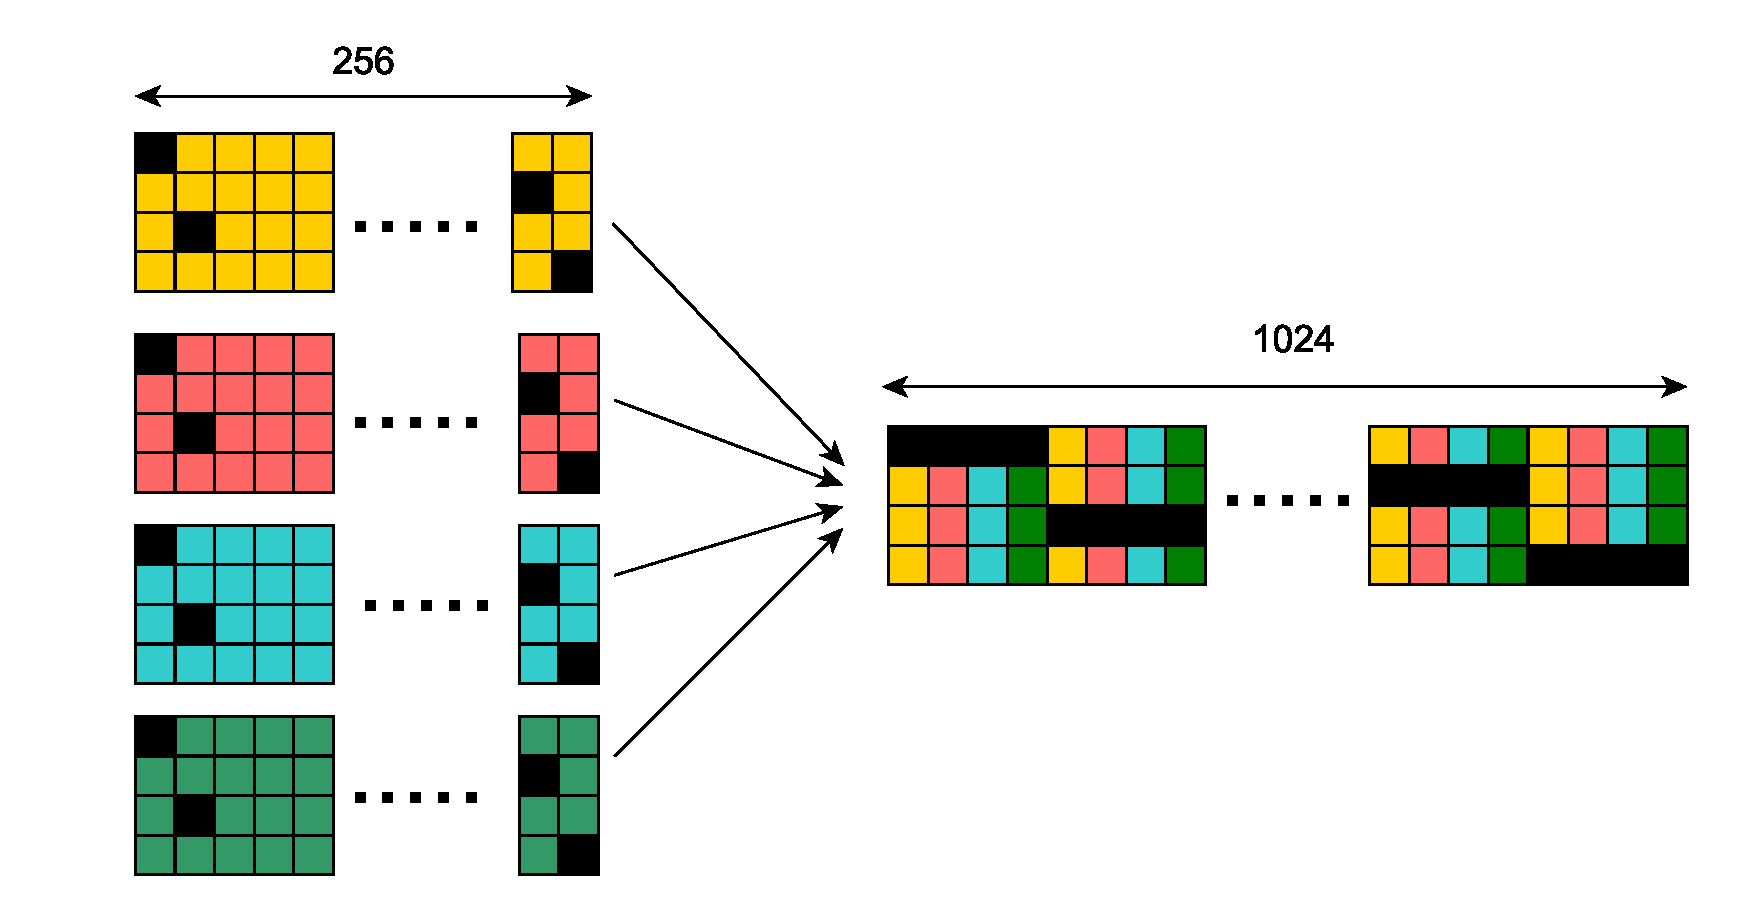
\includegraphics[scale=0.3]{merged_tabular_access.pdf}
			\caption{Memory access patterns for naive and merged tabulation for four hashes. The hash tables are colored with different colors. The accessed locations are shown in black.}
			\label{fig:merged_tabular_access}
	\end{figure}
\end{frame}


\begin{frame}
	\frametitle{Algorithm II: Naive Parallel Count-Min Sketch}
	\begin{algorithm}[H]
		\small
		%\caption{\textsc{Naive-Parallel-CMS}} 
		\SetAlgoNoLine
		\KwIn{  $\epsilon$: error factor, $\delta$: error probability \\
			\hspace*{8ex}${\tt s}[.]$: a stream with $N$ elements from $n$ distinct elements \\ 
			\hspace*{8ex}$h_i(.)$: pairwise independent hash functions where for \\ 
			\hspace*{13.5ex}$1\leq i \leq d$,  $h_i$: $\mathcal{U} \rightarrow \{1,\cdots,w\}$ and $w = \lceil e/\epsilon \rceil$\\
			\hspace*{7.7ex}$\tau$: no threads\\ }
		\KwOut{ ${\tt cms}[.][.]$: a $d \times w$ counter sketch where $d = \lceil 1/\delta \rceil$ \\
		}
		Reset all the ${\tt cms}[.][.]$ counters to 0 (as in Algorithm~\ref{alg:cms_construct}).\\
		\For{$i\leftarrow 1$ \KwTo $N$ {\bf in parallel}}{
			$x  \leftarrow s[i]$\\
			${\tt hashes}[.] \leftarrow$ {\sc MergedHash}($x$)
			
			\For{$j\leftarrow 1$ \KwTo $d$}{
				$col \leftarrow {\tt hashes}[j] $ \\
				${\tt cms}$[j][$col$] $ \leftarrow {\tt cms}$[j][$col$] $ +1$ (\em{must be a critical update})
			}
		}
		\label{alg:cms_construct_par_nobuf}
	\end{algorithm} 	
\end{frame}

\begin{frame}
	\frametitle{Naive Parallel Count-Min Sketch}
	\begin{itemize}
		\item In case a single sketch is used, the naive approach requires a significant synchronization overhead;
		\item In addition, these memory accesses are probable causes of false sharing.
		\vspace*{1ex}
		
		\noindent\rule{10cm}{0.4pt}

		\item Since sketches are combinable, each thread can process a different part of the data to construct a partial CMS.
		\begin{itemize}
		\item These partial sketches can be combined by adding the counter values in the same locations.
		\item Although this approach requires no synchronization, the memory usage increases with increasing number of threads.
		\end{itemize}
	\end{itemize}
\end{frame}

\begin{frame}
\frametitle{Buffered Parallel Count-Min Sketch}
We propose a \textit{buffered parallel} execution% to alleviate the mentioned issues; we
\begin{itemize}
	\item Divide the data into batches and
	\item Process a single batch in parallel in two phases
		\begin{itemize}
		\item{Perform all hash computations for this batch}
		\item{Perform all CMS updates for this batch}
		\end{itemize}
\end{itemize}
\vspace*{1ex}
For a $b$-element batch, the first phase requires a buffer of size $b \times d$ to store the hash values. i.e., column ids. 
Such a buffer allows us to use merged tabulation effectively during the first phase. 
\\
\vspace*{2ex}
The counters in a row are updated by the same
thread hence, there will be no race conditions and probably much less false sharing.
\end{frame}

\begin{frame}
	\frametitle{Algorithm III: Buffered Parallel Count-Min Sketch}
	\renewcommand{\baselinestretch}{0.9}
 \begin{algorithm}[H]
  	\small
  	%\caption{\textsc{Buffered-Parallel-CMS}} 
  	%\KwIn{  $\epsilon$: error factor, $\delta$: error probability \\
	% 	  \hspace*{7ex}${\tt s}[.]$: a stream with $N$ elements from $n$ distinct elements \\ 
%		  \hspace*{7ex}$h_i(.)$: pairwise independent hash functions where for \\ 
%		  \hspace*{13ex}$1\leq i \leq d$,  $h_i$: $\mathcal{U} \rightarrow \{1,\cdots,w\}$ and $w = \lceil e/\epsilon \rceil$\\
%		  \hspace*{7ex}$b$: batch size (assumption: divides $N$)\\
%		  \hspace*{7ex}$\tau$: no threads (assumption: divides $d$)\\ }
%	 \KwOut{ ${\tt cms}[.][.]$: a $d \times w$ counter sketch where $d = \lceil 1/\delta \rceil$ \\
%	 }
		Reset all the ${\tt cms}[.][.]$ counters to 0 (as in Algorithm~\ref{alg:cms_construct})\\[5pt]
		
		
		\For{$i\leftarrow 1$ \KwTo $N/b$}{
			$j_{end} \leftarrow i \times b$	 
			$j_{start} \leftarrow j_{end} - b + 1$
			
			\For{$j\leftarrow j_{start}$ \KwTo $j_{end}$ {\bf in parallel}}{
				$x  \leftarrow {\tt s}[j]$\\
				$\ell_{end} \leftarrow j \times d$\\
				$\ell_{start} \leftarrow \ell_{end} - d + 1$\\
				${\tt buf}[\ell_{start}, \cdots, \ell_{end}] \leftarrow$ {\sc MergedHash}($x$)
			}
			
			{{\bf Synchronize} the threads, e.g., with a {\em barrier}}
			
			\For{$t_{id}\leftarrow 1$ \KwTo $\tau$ {\bf in parallel}}{
				\For{$j\leftarrow 1$ \KwTo $b$ }{
					$nrows \leftarrow d / \tau$\\
					$r_{end} \leftarrow t_{id} \times nrows$\\
					$r_{start} \leftarrow r_{end} - nrows + 1$\\
					\For{$r\leftarrow r_{start}$ \KwTo $r_{end}$ }{
						$col \leftarrow {\tt buf}[((j-1) \times d) + r]$\\
						${\tt cms}[r][col] \leftarrow {\tt cms}[r][col] +1$
			}
			}
			}

			}
	\label{alg:cms_construct_par}
\end{algorithm} 	
\renewcommand{\baselinestretch}{1}
			
\end{frame}
 
\begin{frame}
	\frametitle{Managing Heterogeneous Cores}
	\begin{itemize}
		\item When the cores are homogeneous, Algorithm 3 works efficiently with static scheduling since, each thread performs the same amount of merged hashes and counter updates.
		\noindent\rule{10cm}{0.4pt}

		\item Some SBCs use the {\em big.LITTLE} architecture equipped with power-hungry fast cores, as well as energy-saving slow cores.
		\begin{itemize}
		\item Tasks can be swapped between these cores on the fly.
		\end{itemize}
		\item The first inner loop (hashing) can be dynamically  scheduled.
		\item The same technique is not applicable to the second inner loop where the counter updates are performed: when the fast cores are done
		with the updates, the slow cores will still be working.
	\end{itemize}
\end{frame} 

\begin{frame}
		\frametitle{Managing Heterogenous Cores}
		To alleviate these problems, we propose to pair a slow core with a fast one and
		make them update two rows in an alternating fashion.
		
		\begin{figure}[H]
			%\begin{minipage}[c]{0.55\textwidth}
				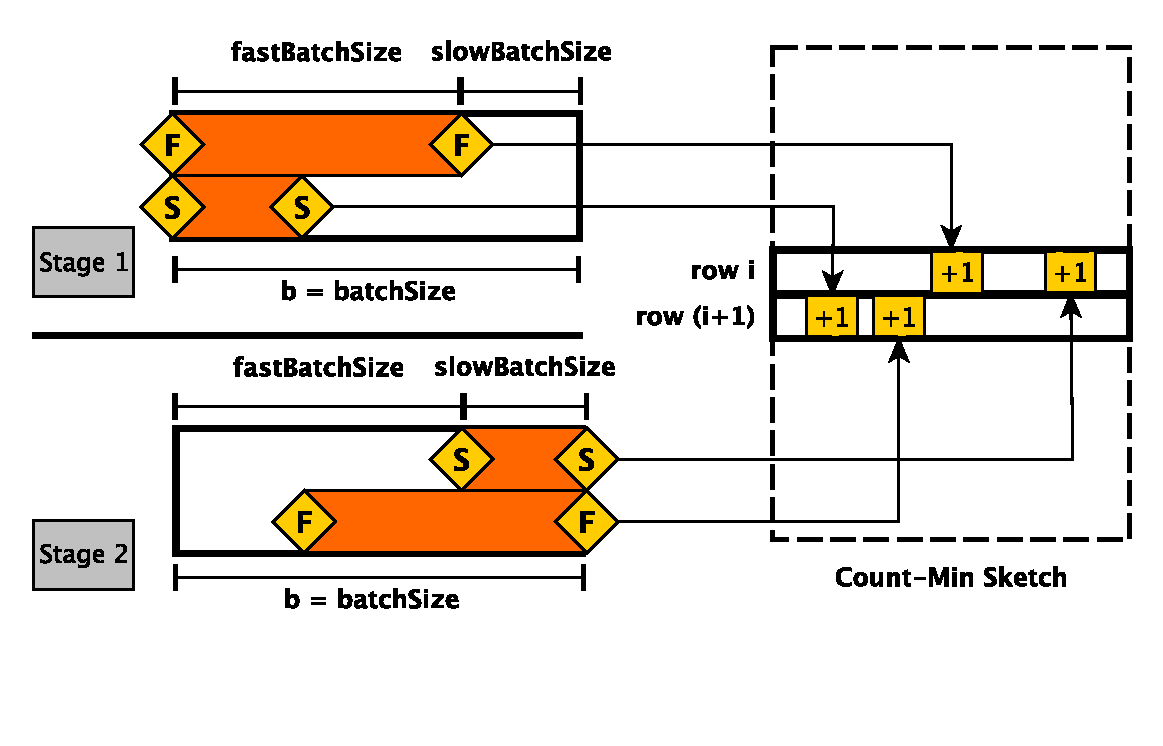
\includegraphics[scale=0.45]{fastslow.pdf}
			%\end{minipage}\hfill\hfill\hfill
			%\begin{minipage}[c]{0.42\textwidth}
				\caption{\small{For a single batch, rows $i$ and $i+1$ of CMS are updated by a fast/slow core pair in two stages. The fast core first processes row $i$ and the slow processes row $i+1$. Then, they exchange the rows and complete the remaining updates for the current batch.}}
				\label{fig:fastslow}
			%\end{minipage}
			%\vspace*{-4ex}
		\end{figure}
\end{frame}

\begin{frame}
	\frametitle{Managing Heterogenous Cores}
	\begin{itemize}
	\item	In both stages, the faster threads process $fastBatchSize$ items\\ and the slower ones process $slowBatchSize$ items where\\ 
	%\vspace{0.2cm}
	$b = fastBatchSize + slowBatchSize.$%\vspace*{-2ex}
	%\vspace{0.4cm}
	\item To avoid the overhead of dynamic scheduling and propose a generic solution, we start with %\\
	\begin{align*}
	fastBatchSize = b/2 \\ %and \\
	slowBatchSize = b/2 %\\
	 \end{align*}
	 and by measuring the time spent by the cores, we dynamically adjust them to distribute the workload among all the cores as fairly as possible. 
	\end{itemize}
\end{frame}

\begin{frame}
	\frametitle{Managing Heterogenous Cores}
	\begin{itemize}
	\item Let $t_F$ and $t_S$ be the times spent by a fast and slow core, respectively, on average.
	\item Let $s_F = \frac{fastBatchSize}{t_F}$ and $s_S = \frac{slowBatchSize}{t_S}$ be the speed of these cores for the same operation, e.g., hashing, CMS update etc.
	\item Then solve the equation $\frac{fastBatchSize + x}{s_F} = \frac{slowBatchSize - x}{s_S}$ for $x$ and update the values as 
	\begin{align*}
	fastBatchSize &= fastBatchSize + x\\
	slowBatchSize &= slowBatchSize - x
	\end{align*}
	for the next batch.
	\end{itemize}
\end{frame}


\begin{frame}
	\frametitle{Experimental Setup}
	We perform experiments on the following three architectures: 
	\begin{itemize}
		\item {\bf Xeon} is a server running on 64 bit CentOS 6.5 equipped with an Intel Xeon E7-4870 v2 clocked at 2.30 GHz and having 15 cores. Each core has a 32KB L1 and a 256KB L2 cache, and the size of L3 cache is 30MB. 
		\item {\bf Pi} ({\bf Raspberry Pi 3 Model B+}) is a quad-core 64-bit ARM Cortex A-53 clocked at 1.4 GHz equipped with 1 GB LPDDR2-900 SDRAM. Each core has a 32KB L1 cache, and the shared L2 cache size is 512KB.
		\item {\bf Odroid} ({\bf Odroid XU4}) is an octa-core multi-processor. There are four 2Ghz A15 cores and four A7 1.4Ghz cores and a 2GB LPDDR3 RAM. Each core has a 32KB L1 cache. The fast cores have a shared 2MB L2 cache and slow cores have a shared 512KB L2 cache. 
	\end{itemize}
\end{frame}

\begin{frame}
	\frametitle{Experimental Setup}
	\begin{itemize}
		\item We use C++ and OpenMP. We use {\tt gcc 5.3.0} on {\bf Xeon}. On {\bf Pi} and  {\bf Odroid}, the {\tt gcc} version is {\tt 6.3.0} and {\tt 7.3.0}, respectively. For all architectures, {\tt -O3} optimization flag is also enabled.
		\item We used {\em Zipfian} distribution~\cite{Zipf1935} to generate datasets. Many data in real world such as number of paper citations, file transfer sizes, word frequencies etc. fit to a Zipfian distribution with the shape parameter around $\alpha = 1$.
		%\item The distribution is a common choice for the studies in the literature to benchmark the estimation accuracy of data sketches.
		\begin{itemize}
		\item To cover the practice better, we used the shape parameter $\alpha \in \{1.1, 1.5\}$.
		\end{itemize}
	\end{itemize}
\end{frame}

\begin{frame}
	\frametitle{Experimental Setup}
	\begin{itemize}
	\item We use $\epsilon \in \{10^{-3}, 10^{-4}, 10^{-5}\}$ and $\delta = 0.003$ to generate small, medium and large $d \times w$ sketches  where the number of columns is chosen as the first prime after $2/\epsilon$. 
	\item The sketches have $w = \{2003, 20071, 200003\}$ columns and $d = \lceil \log_2(1/\delta) \rceil = 8$ rows. 
	\item For the experiments on {\bf Xeon}, we choose $N = 2^{30}$ elements from a universal set $\mathcal{U}$ of cardinality $n = 2^{25}$. 
	\item For {\bf Pi} and   {\bf Odroid}, we use $N = 2^{25}$ and $n = 2^{20}$. 
	\item For all architectures, we used $b = 1024$ as the batch size. 
	\item Each data point in the tables and charts given below is obtained by averaging ten runs.
	\end{itemize}
\end{frame}


\begin{frame}
	\frametitle{Experimental Results}
\begin{itemize} 
\item MT uses the multi-sketch, i.e., one-sketch-per-core, approach as suggested in the literature, 
\item MT+ is the MT-variant with merged tabulation, 
\item ST+ is the proposed single-sketch parallelization scheme,
\item ST++ is the ST+ variant using the load-balancing scheme for heterogeneous cores.
\end{itemize} 
\end{frame}

\begin{frame}
	\frametitle{Experimental Results}
	\setbeamerfont{caption}{size=\tiny}
	\begin{figure}[H]\hspace*{-12mm}
			\begin{minipage}[c]{0.7\textwidth}
			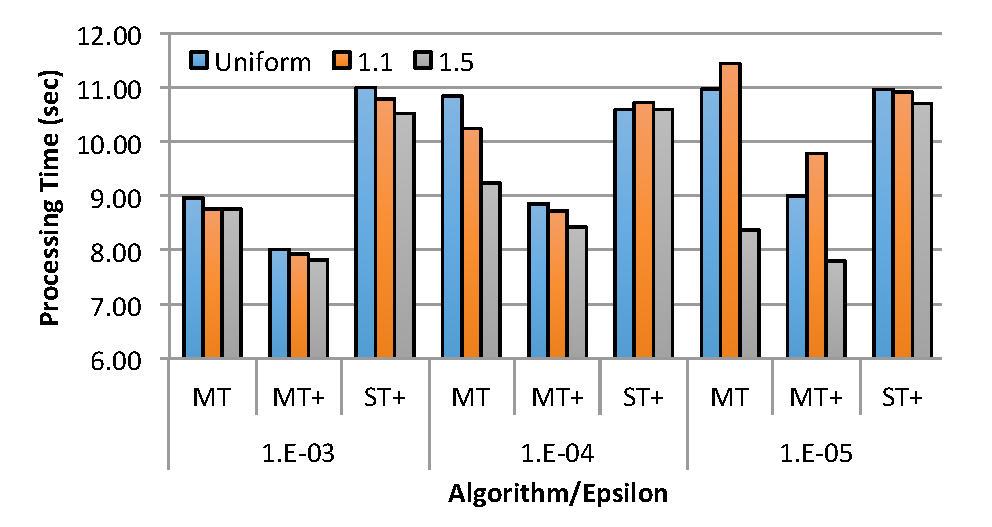
\includegraphics[scale=0.47]{main_1_8.pdf}
		\end{minipage}
		\begin{minipage}[c]{0.25\textwidth} \hspace*{2ex}{{\bf Xeon} - 8 cores} \end{minipage}

		\begin{minipage}[c]{0.7\textwidth}
			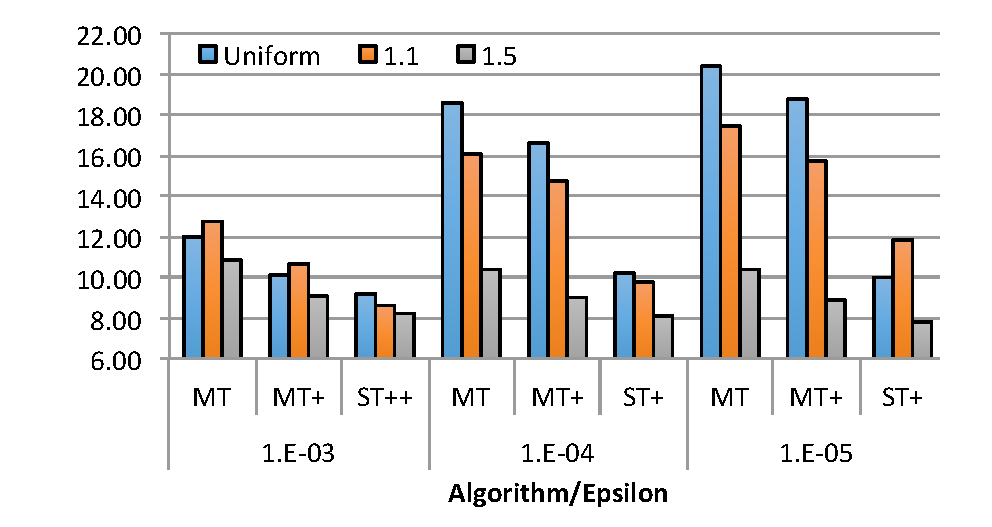
\includegraphics[scale=0.45]{main_2_4.pdf}
		\end{minipage}
		\begin{minipage}[c]{0.25\textwidth} {{\bf Pi} - 4 cores} \end{minipage}
		\end{figure}
\end{frame}

\begin{frame}
	\frametitle{Observations}
	On {\bf Xeon}
	\begin{itemize}
		\item Although ST+ uses much less memory, its performance is not good due to all the time spent while buffering and synchronization.
		\item The last level cache size on  {\bf Xeon} is 30MB; considering the largest sketch we have is 6.4MB~(with 4-byte counters), {\bf Xeon} does not suffer from its cache size and MT+ indeed performs much better than ST+.
	\end{itemize}
	On {\bf Pi}
	\begin{itemize}
		\item With a $512$KB last-level cache, the proposed technique ~(ST+) significantly improves the performance, and while doing that, it uses significantly much less memory.
	\end{itemize}

\end{frame}


\begin{frame}
	\frametitle{Managing Heterogenous Cores}
	 We propose to compute the fast/slow batch sizes only for a few batches and use the average value for the later batches {\it to obtain a generic and dynamic solution on all archotectures}. 
	 %We applied this technique both for hashing and counter update phases of the proposed buffered CMS generation algorithm.
	
	\vspace{-4mm}
	\begin{figure}[H]
		\begin{minipage}[c]{0.49\textwidth}
			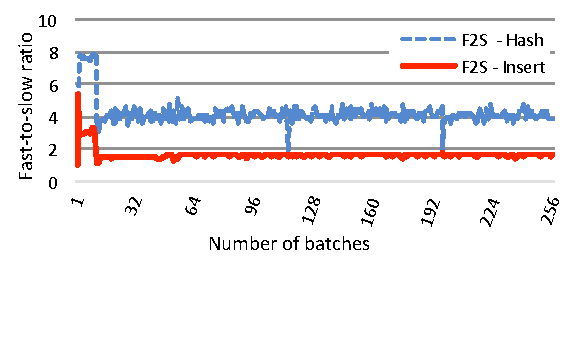
\includegraphics[width=\linewidth]{f2s-small.pdf}
			\caption{{\bf small} CMS on {\bf Odroid}}
			\label{fig:fs-small}
		\end{minipage}\hspace*{3ex}
		\begin{minipage}[c]{0.49\textwidth}
			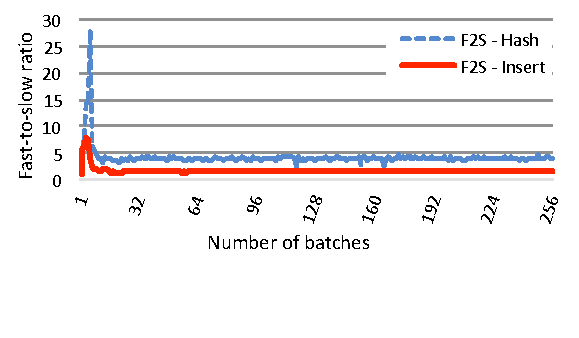
\includegraphics[width=\linewidth]{f2s-big.pdf}
			\caption{{\bf medium} CMS on {\bf Odroid}}
			\label{fig:fs-large}
		\end{minipage}
		
		\caption{\small{Fast-to-slow ratio $F2S = \frac{fastBatchSize}{slowBatchSize}$ of hashing and CMS update for consecutive batches and for small~(left) and medum~(right) sketches.}}
		\label{fig:load}
		\vspace*{-6ex}
	\end{figure}
	
\end{frame}


\begin{frame}
	\frametitle{Experimental Results}
	\setbeamerfont{caption}{size=\tiny}
	\begin{figure}[H]\hspace*{-12mm}
		
		\begin{minipage}[c]{0.7\textwidth}
			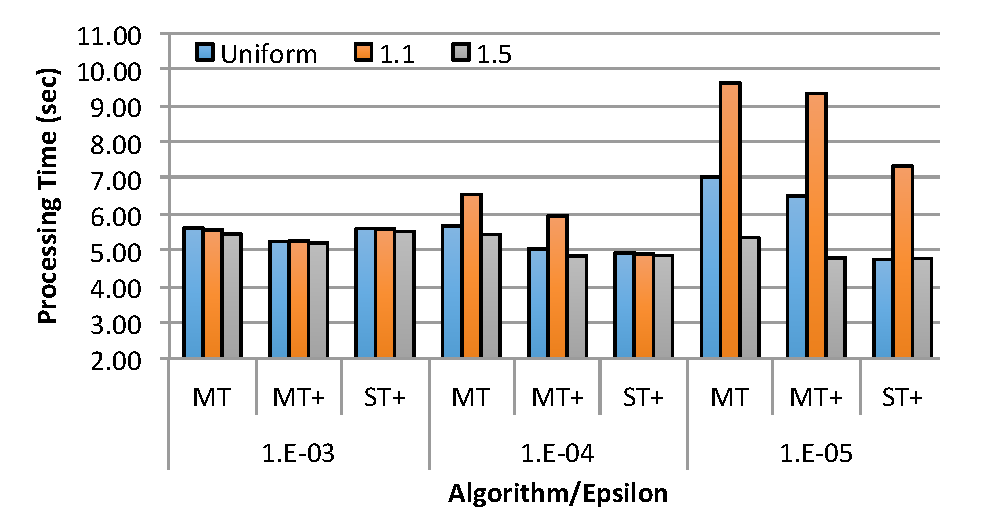
\includegraphics[scale=0.40]{main_3_4.pdf}
		\end{minipage}
		\begin{minipage}[c]{0.25\textwidth} {{\bf Odroid} - 4 cores} \end{minipage}

		\begin{minipage}[c]{0.7\textwidth}
			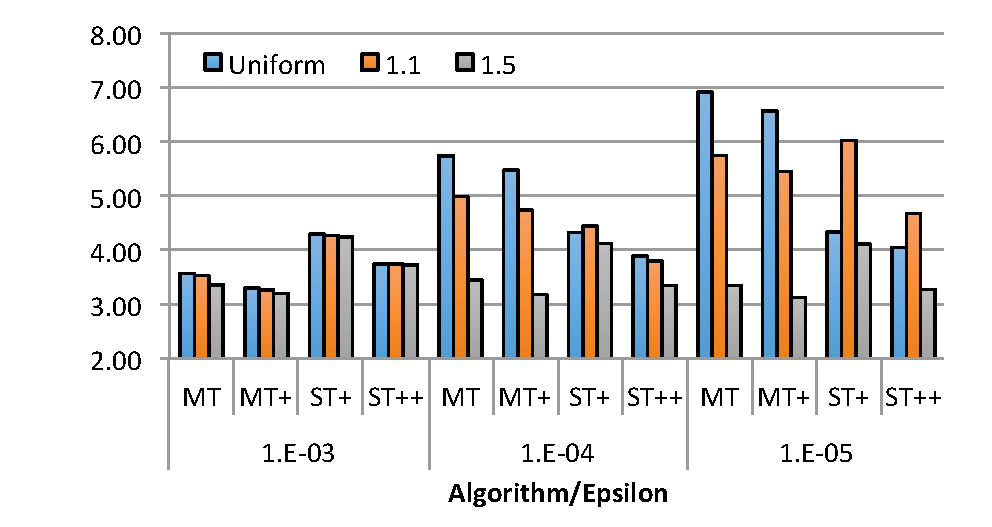
\includegraphics[scale=0.43]{main_3_8.pdf}
		\end{minipage}
		\begin{minipage}[c]{0.25\textwidth} {{\bf Odroid} - 8 cores} \end{minipage}
		\end{figure}
\end{frame}



\begin{frame}
	\frametitle{Experimental Results Discussion}
	On {\bf Odroid}
	\begin{itemize}
		\item A performance increase similar to {\bf Pi} is visible for medium~(640KB) and especially large~(6.4MB) sketches when only the fast cores with a 2MB last-level cache are used.
		\item ST++, the single-table approach both with merged tabulation and load balancing, is always better than ST+.
		\item When $\tau = 8$, with the small 512KB last-level cache for slower cores, the ST++ improves MT+ much better.
		\item Overall, smart load distribution increases the efficiency by $15\%$--$30\%$ for $\tau = 8$ threads.
	\end{itemize}
\end{frame}

\begin{frame}
	\frametitle{Experimental Results Discussion}
	On {\bf Distribution}
	\begin{itemize}
		\item The performance of the algorithms vary with respect to the distribution.
		\item For uniform and Zipfian($1.1$), the execution times tend to increase with sketch sizes.
		\item Nevertheless, for $\alpha = 1.5$, sketch size does not have a huge impact on the performance, since only the {\em hot} counters of the most frequent items are frequently updated.
		\item Although each counter has the same chance to be a hot counter, the effective sketch size reduces significantly especially for large sketches.
		\begin{itemize}
			\item This is the reason of being much faster for $\alpha = 1.5$.
		\end{itemize}
	\end{itemize}
\end{frame}



\begin{frame}[fragile]
	\frametitle{Thanks!}
	Thanks for your time.\\
	\vspace{3mm}
	%\url{http://people.sabanciuniv.edu/kaya}
	
	\vspace{5mm}
	\textcolor{darkred}{More Information}
	\begin{itemize}
		\item One Table to Count Them All: Parallel Frequency Estimation on Single-Board Computers, {\it Euro-Par: 25th International European Conference on Parallel and Distributed Computing}, 26-30 August, 2019, G\"{o}ttingen, Germany  \\
	\end{itemize}
	
\end{frame}


\begin{frame}[allowframebreaks]
\frametitle{References}
\bibliographystyle{plain}
\bibliography{sketch}
\end{frame}



 
\end{document}